\section{The Silicon Tracker}
\label{sec:tracker}
At the heart of CMS is one of the world's largest silicon detectors: the silicon tracker (Fig.~\ref{fig:tracker_real}).
It is the subdetector closest to the \pp interaction point.
The main goal of the silicon tracker is not to stop the outgoing particles but to very precisely measure the hits from the charged particles as they pass through it.
The tracker also assists with vertex identification, differentiating between primary and secondary vertices, the latter of which often comes from $B$-meson decays.
When multiple \pp collisions occur within the same BX, the tracker distinguishes between \pp vertices with a resolution of about 15--20\mum.
This is crucial to resolve which outgoing particles came from which \pp vertex.
The tracker consists of two types of pure silicon detectors: the pixel detector and the strip detector, each of which is described in turn below.
%%%%%%%%%%%%%%%%%%%%
%=== Real image silicon tracker.
\begin{multiFigure}
    \centering
    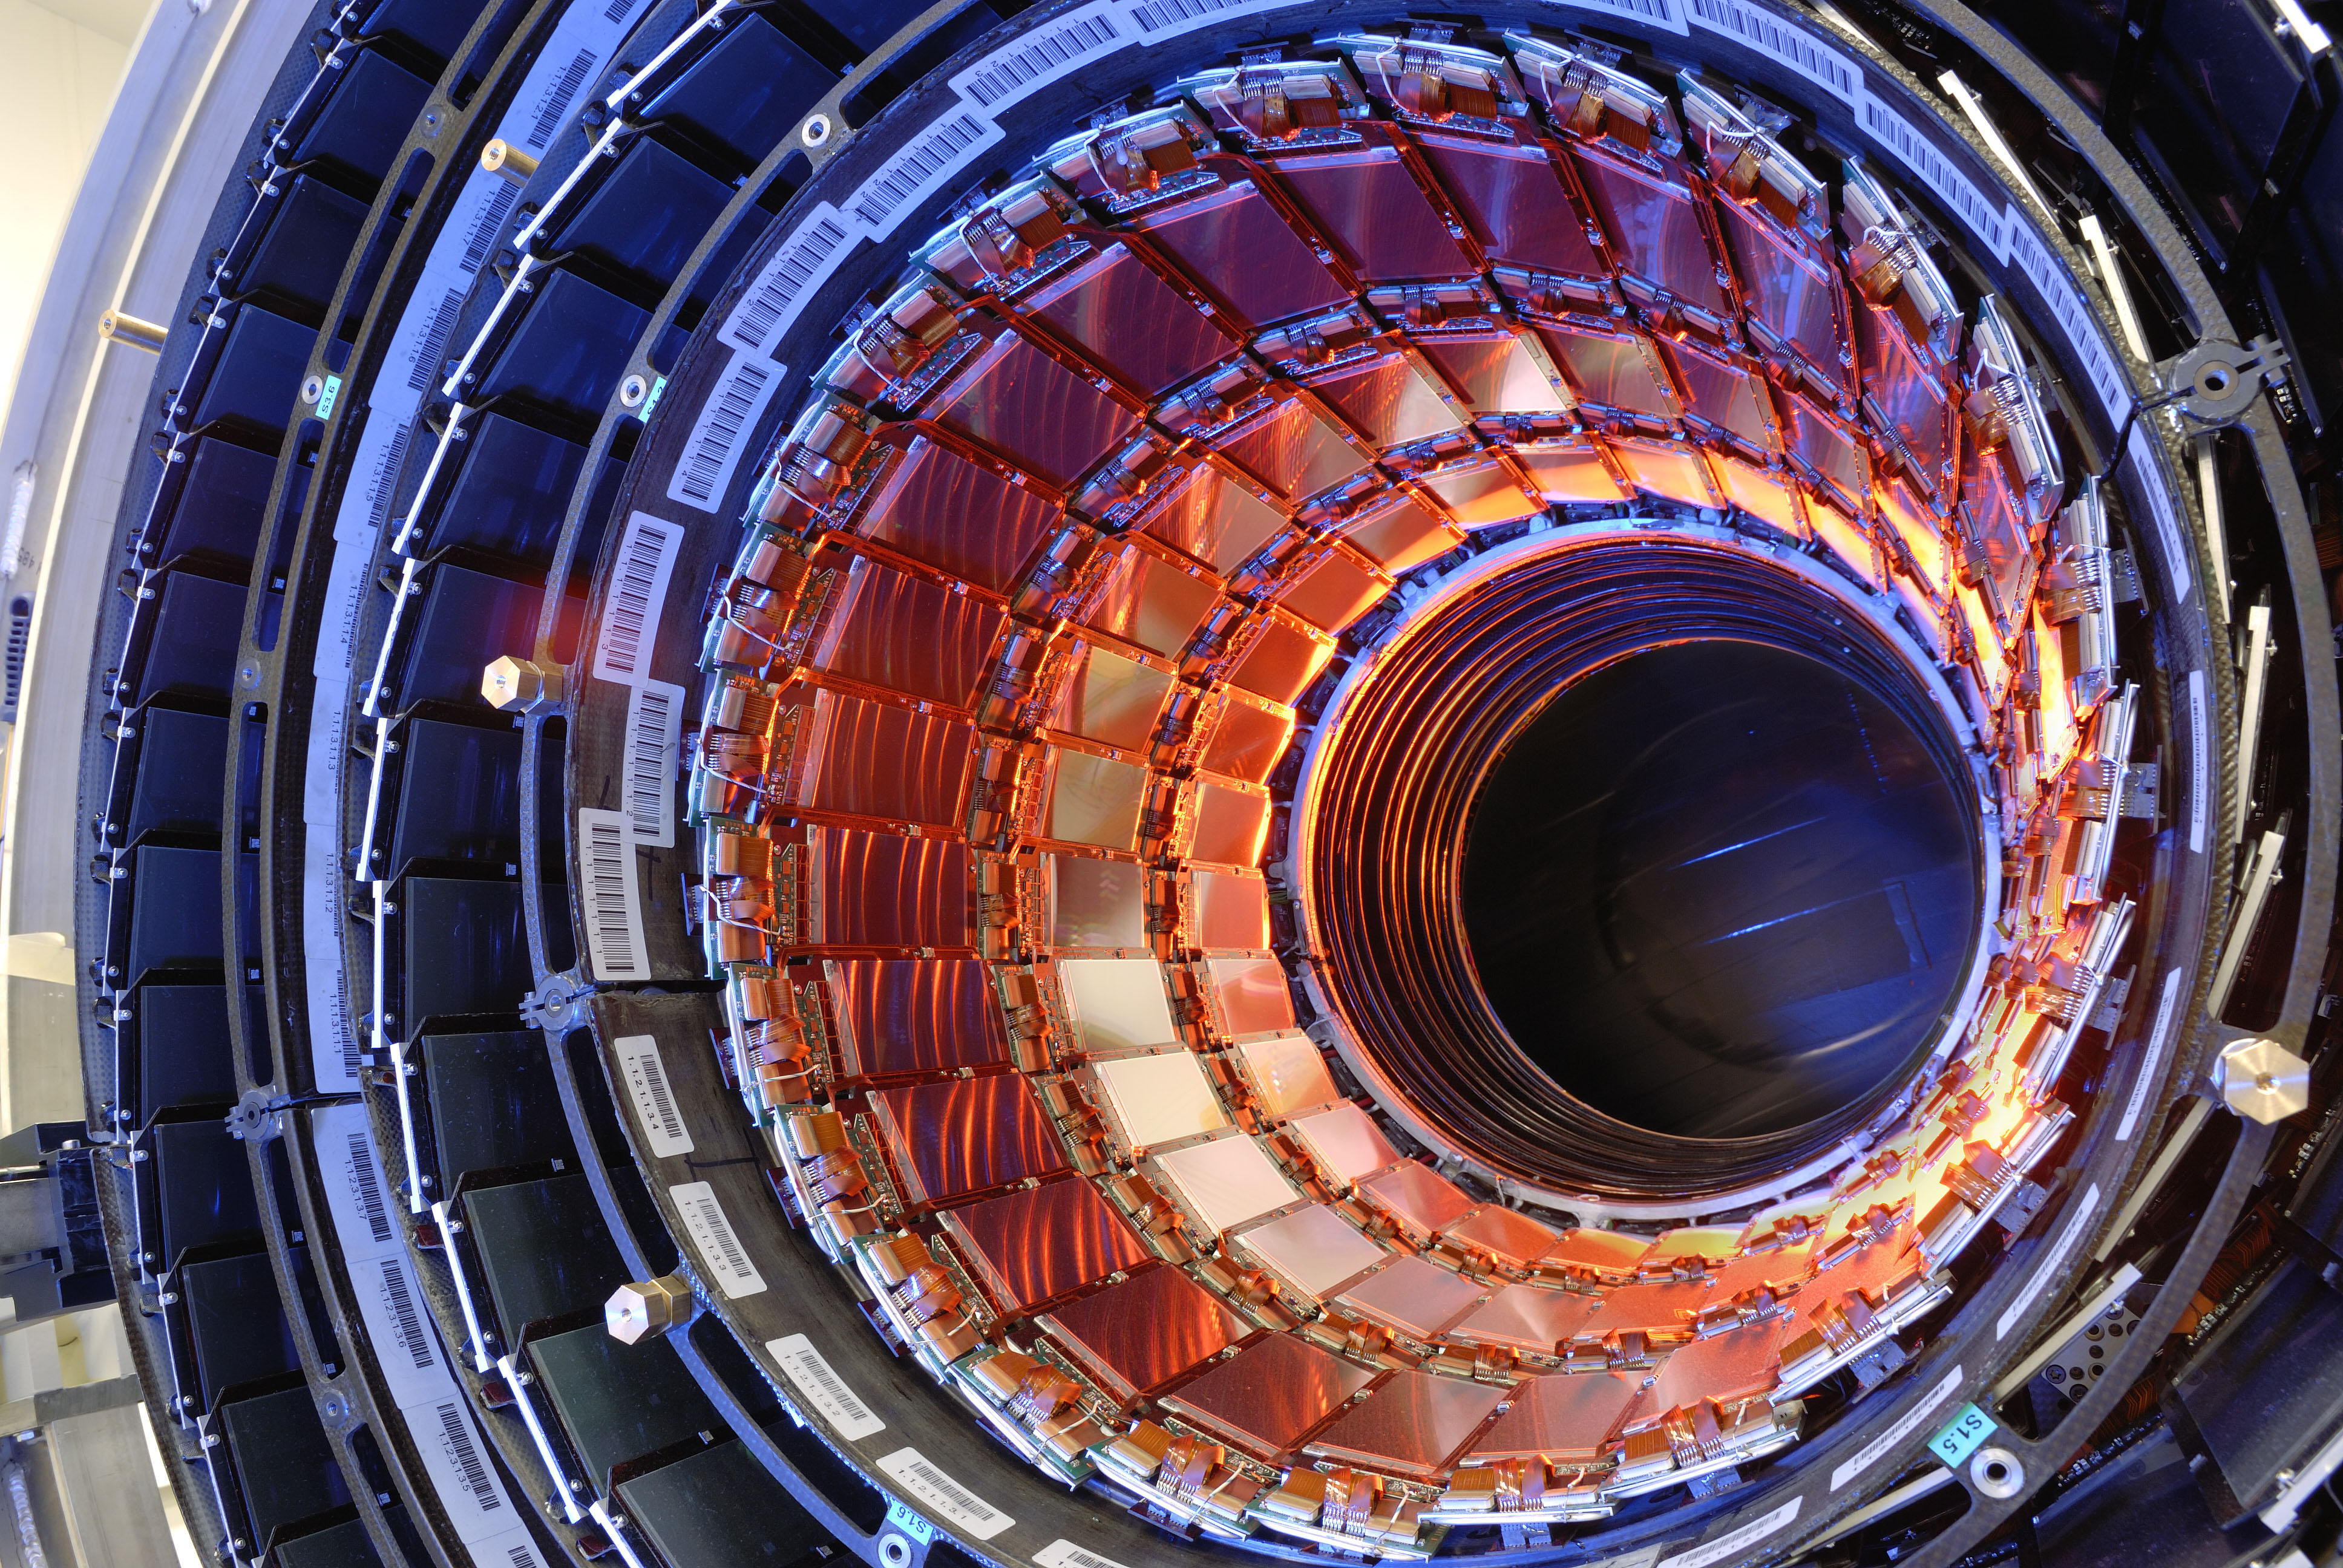
\includegraphics[width=0.8\textwidth]{figures/cms/tracker/silicon_tracker_real.jpg}
    \captionof{figure}
        [The real silicon tracker at the center of CMS]
        {The real silicon tracker at the center of CMS. Figure taken from~\cite{tracker_real}.}
    \label{fig:tracker_real}
\end{multiFigure}
%%%%%%%%%%%%%%%%%%%%

\subsection{The Pixel Detector}
\label{sec:pixel}
After the LHC Run 1 finished, the collider received luminosity upgrades during the 2013--2014 Long Shutdown.
To handle these higher luminosities, the pixel detector was replaced by the CMS Phase-1 pixel detector during the LHC technical stop in 2016--2017.
The upgrades outfitted the pixel detector with four barrel layers and three endcap disks per side, which allowed for particle detection up to $\abseta < 2.5$.
Figure~\ref{fig:pixel_xs_long} shows the changes within the pixel detector before and after the Phase-1 upgrade.
The overall mass of the pixel detector decreased and granted the detector with better tracking capability.
%%%%%%%%%%%%%%%%%%%%
%=== Before/after Phase-1 Upgrade of pixel detector.
\begin{multiFigure}
    \centering
    % \addFigure{0.49}{figures/cms/tracker/silicon_tracker_simulated.png}
    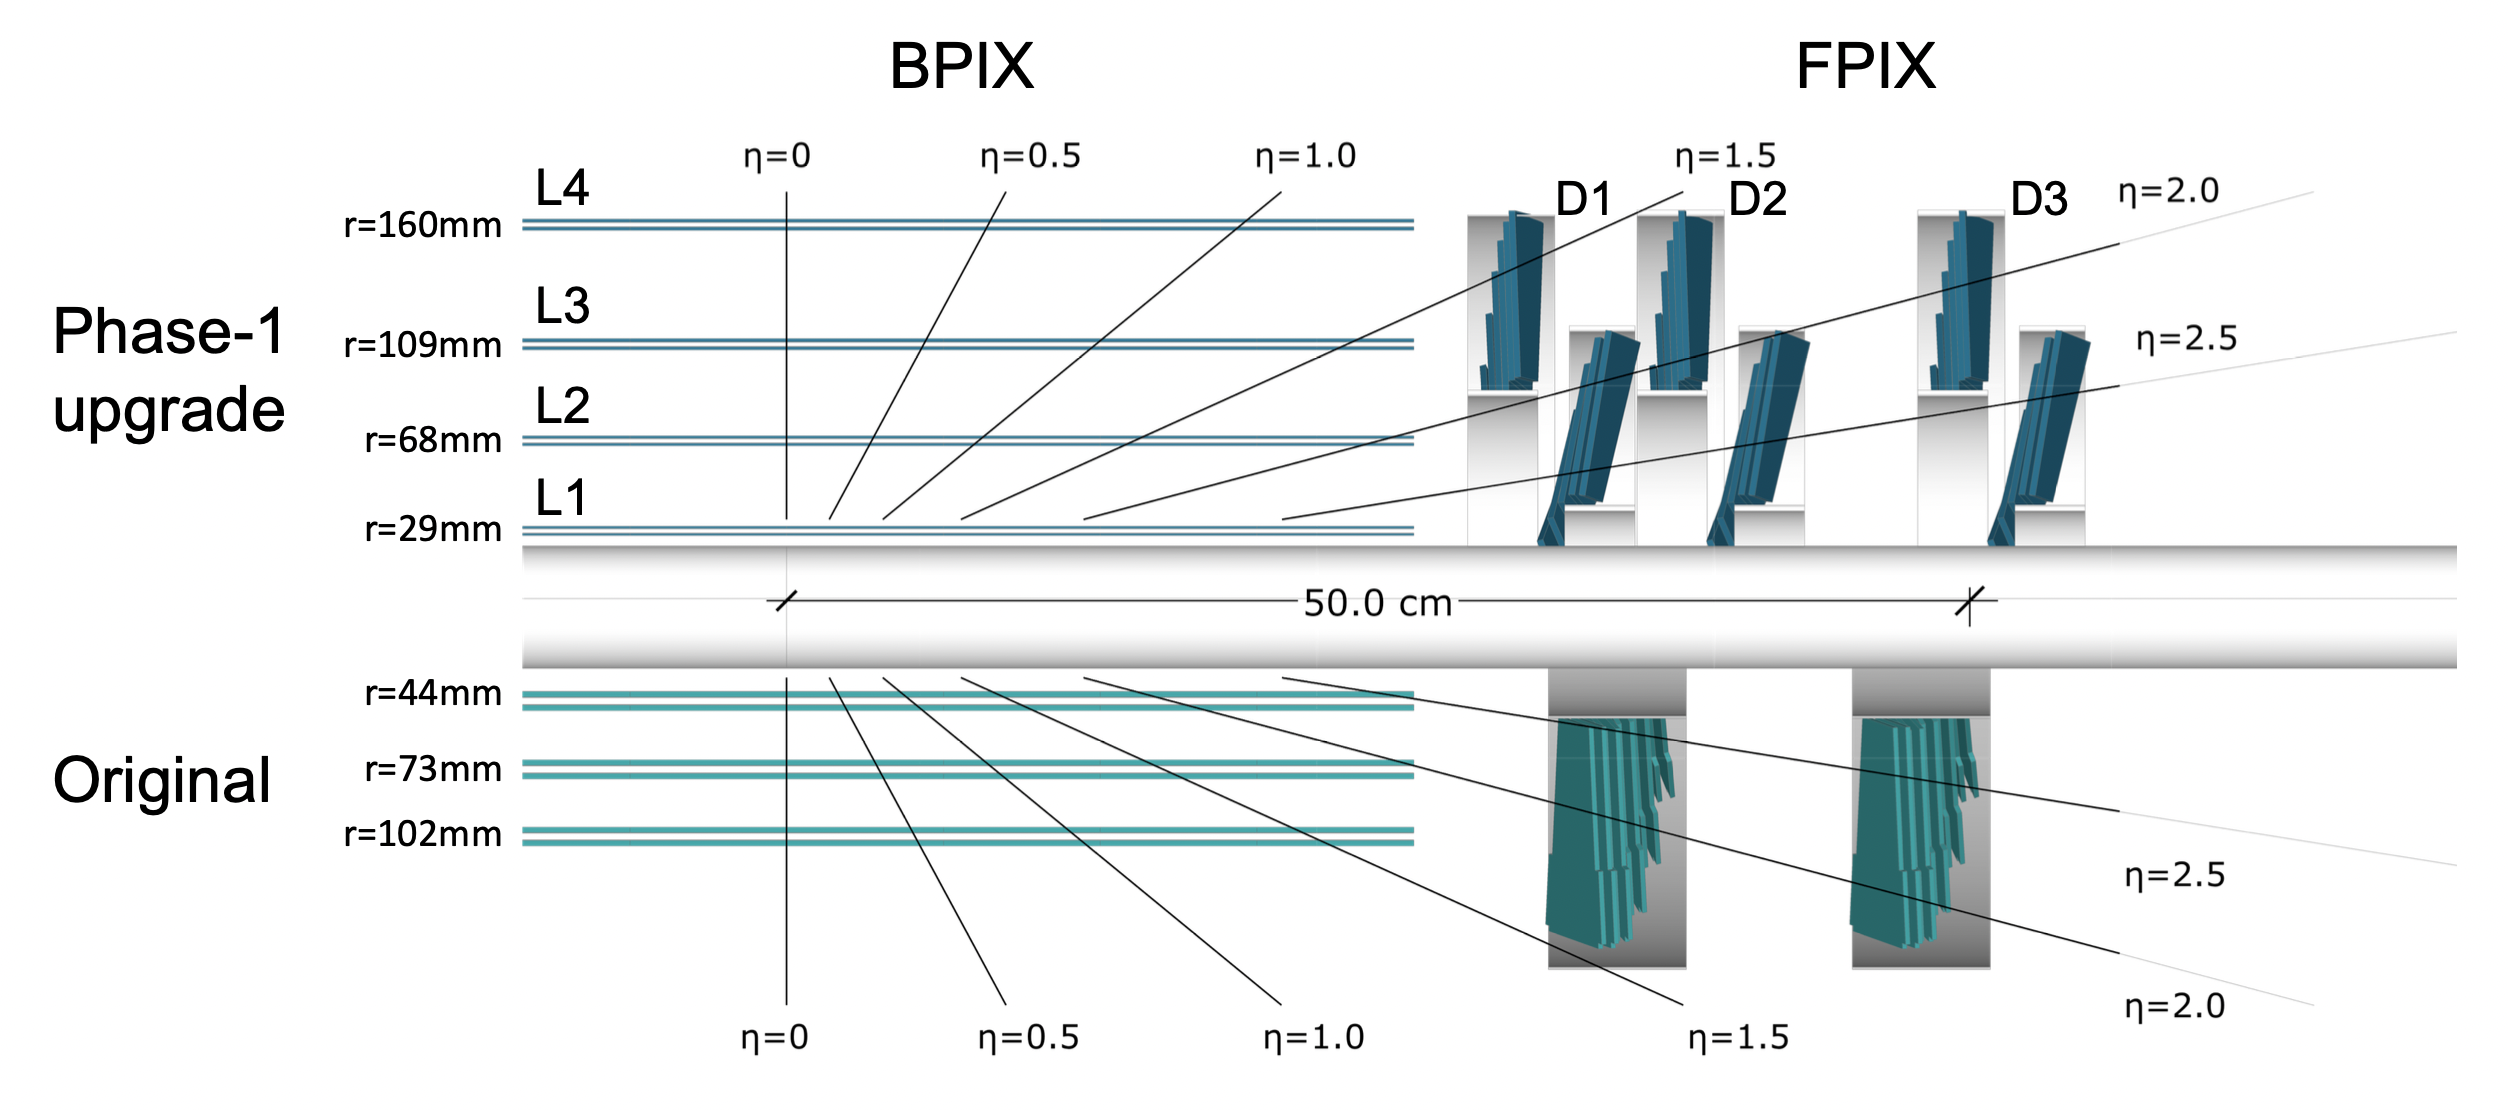
\includegraphics[width=\textwidth]{figures/cms/tracker/pixel_barrel_upgrade.png}
    \captionof{figure}
        [Longitudinal cross section of the Phase-1 pixel detector]
        {Longitudinal cross section of the pixel detector.
        The top-half of the figure shows the pixel detector after the ``Phase-1 upgrade'' (\eg having 4 barrel layers) as compared to its ``Original'' version (with only 3 barrel layers) in the bottom-half of the figure.
        Figure taken from~\cite{pixel_phase1}.}
    \label{fig:pixel_xs_long}
\end{multiFigure}
%%%%%%%%%%%%%%%%%%%%

The innermost part of the silicon tracker is the pixel detector, which is composed of 124 \emph{million} silicon ``pixels''.
A single pixel is 100\mum $\times$ 150\mum and, collectively, they cover a sensitive area of 1.9$\meter^2$.
Because it sits only 29\mm away from the beam pipe, the pixel detector receives the highest particle flux than any other subdetector:
around 10 million particles/$\cmns^2$ per second.

\subsection{The Strip Detector}
\label{sec:strip}
The outer part of the silicon tracker is called the strip detector and has $\approx$10 million detector strips spread across 10 cylindrical layers.
The first 4 layers belong to the tracker inner barrel (TIB) and the remaining 6 layers belong to the tracker outer barrel (TOB), Fig.~\ref{fig:tracker_xs}. 
Both the TIB and TOB have two endcaps associated with them, the TID and TEC, respectively.
Accounting for all of its components, the strip detector is sensitive to 200$\meter^2$.
Figure~\ref{fig:tracker_xs} shows a clearly labeled transverse view of the pixel and strip detectors before the Phase-1 upgrade.
%=== Transverse view of silicon tracker.
\begin{multiFigure}
    \centering
    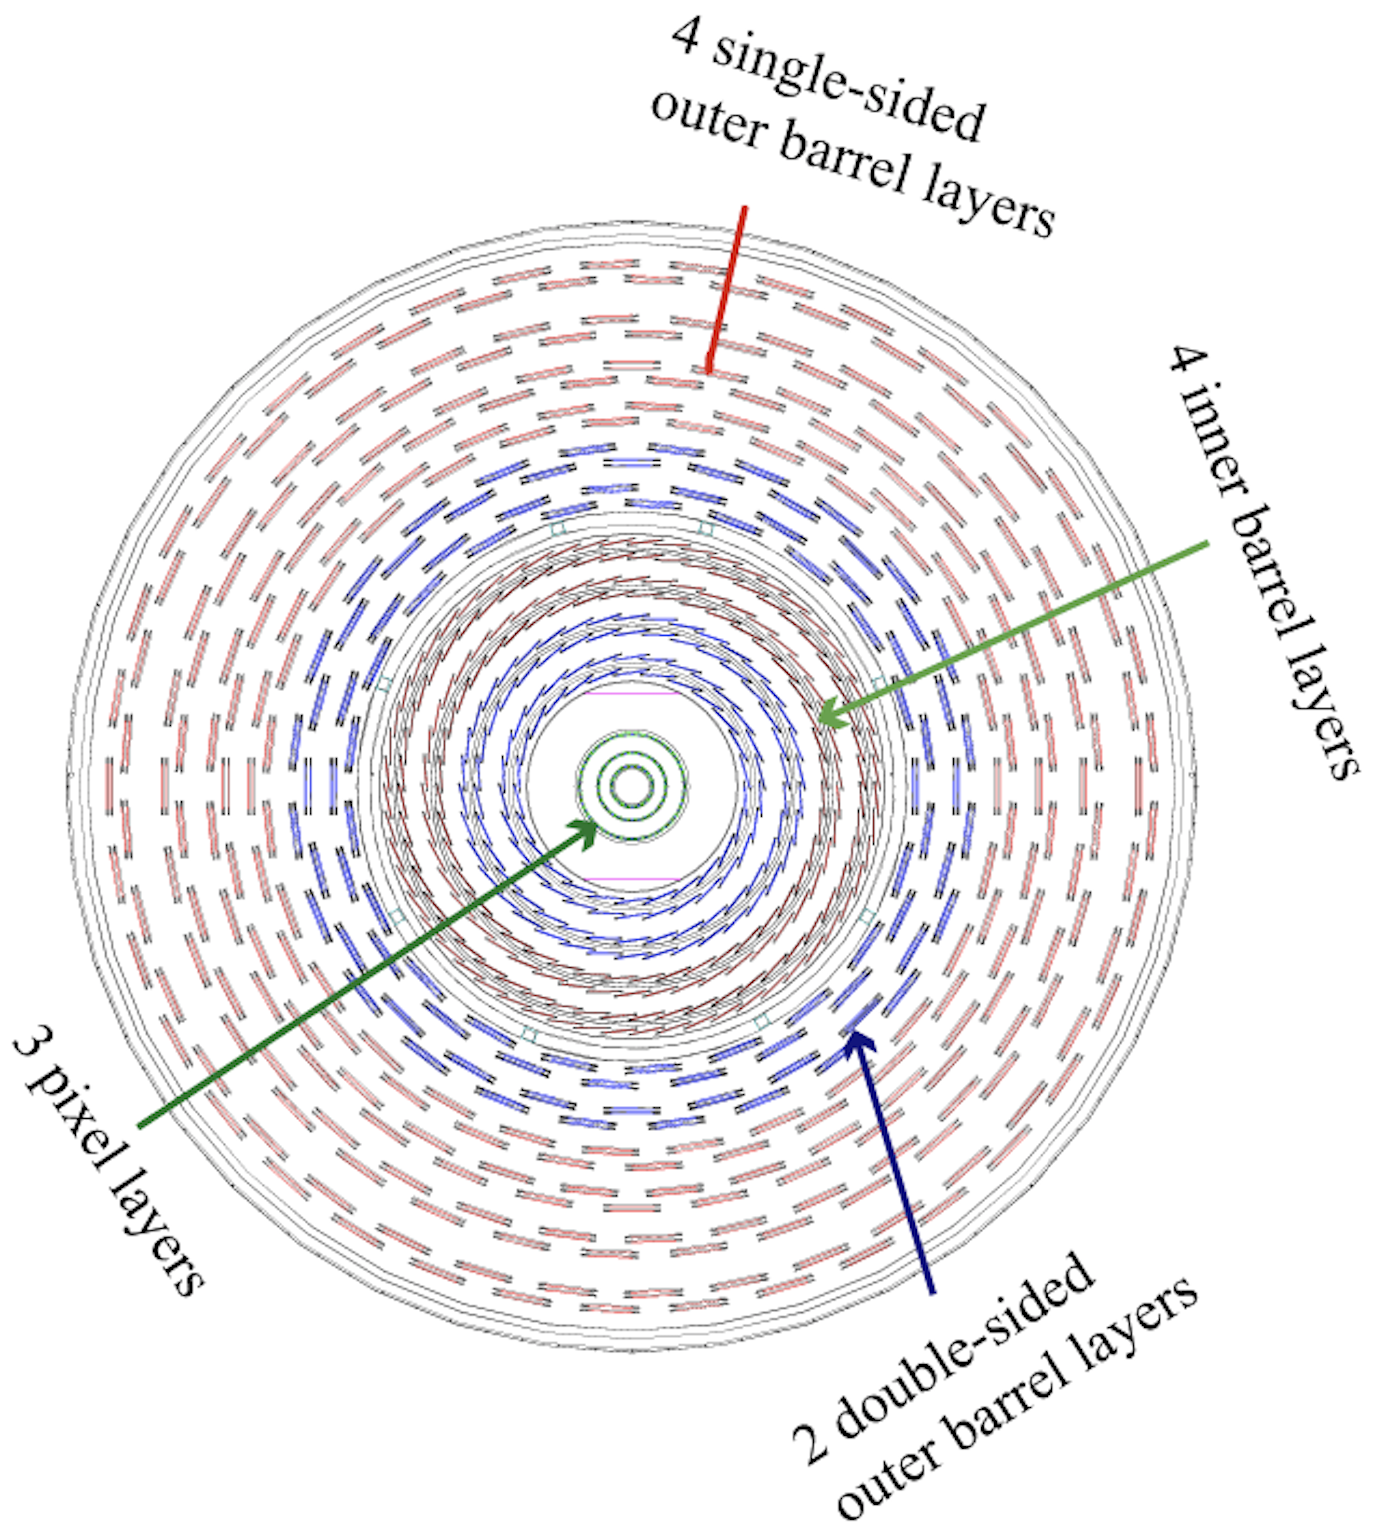
\includegraphics[width=10cm,height=10cm,keepaspectratio]{figures/cms/tracker/silicon_tracker_transverse_view.png}
    \captionof{figure}
        [Transverse view of the silicon pixel and strip detectors]
        {Transverse view of the silicon pixel and strip detectors, explicitly labeling the different tracking layers.
        Note that the inner ``3 pixel layers'' indicates that this image is before the Phase-1 upgrade of the pixel detector.
        Figure taken from~\cite{strip_detector_xs}.}
    \label{fig:tracker_xs}
\end{multiFigure}
%%%%%%%%%%%%%%%%%%%%
